\documentclass[11pt,a4paper]{article}
\usepackage[latin1]{inputenc}
\usepackage{amsmath}
\usepackage{amsfonts}
\usepackage{amssymb}
\usepackage{array}
\usepackage{graphicx}
\usepackage{float}
\author{Jordan Murray}
\title{EECS305 Lab5}
\begin{document}
\begin{center}
\fontsize{24}{12}\selectfont
\textbf{Solutions For Lab 2:}

\textbf{ Model Identification and Transient Response of a DC Servo Motor System }
\end{center}

\section{Procedure}
\textbf{3.1 Model Identification}
The Simulink model Lab2\_Identification was run. A unit step function was given as an input to the DC model block producing the following trajectories:

\begin{figure}[H]
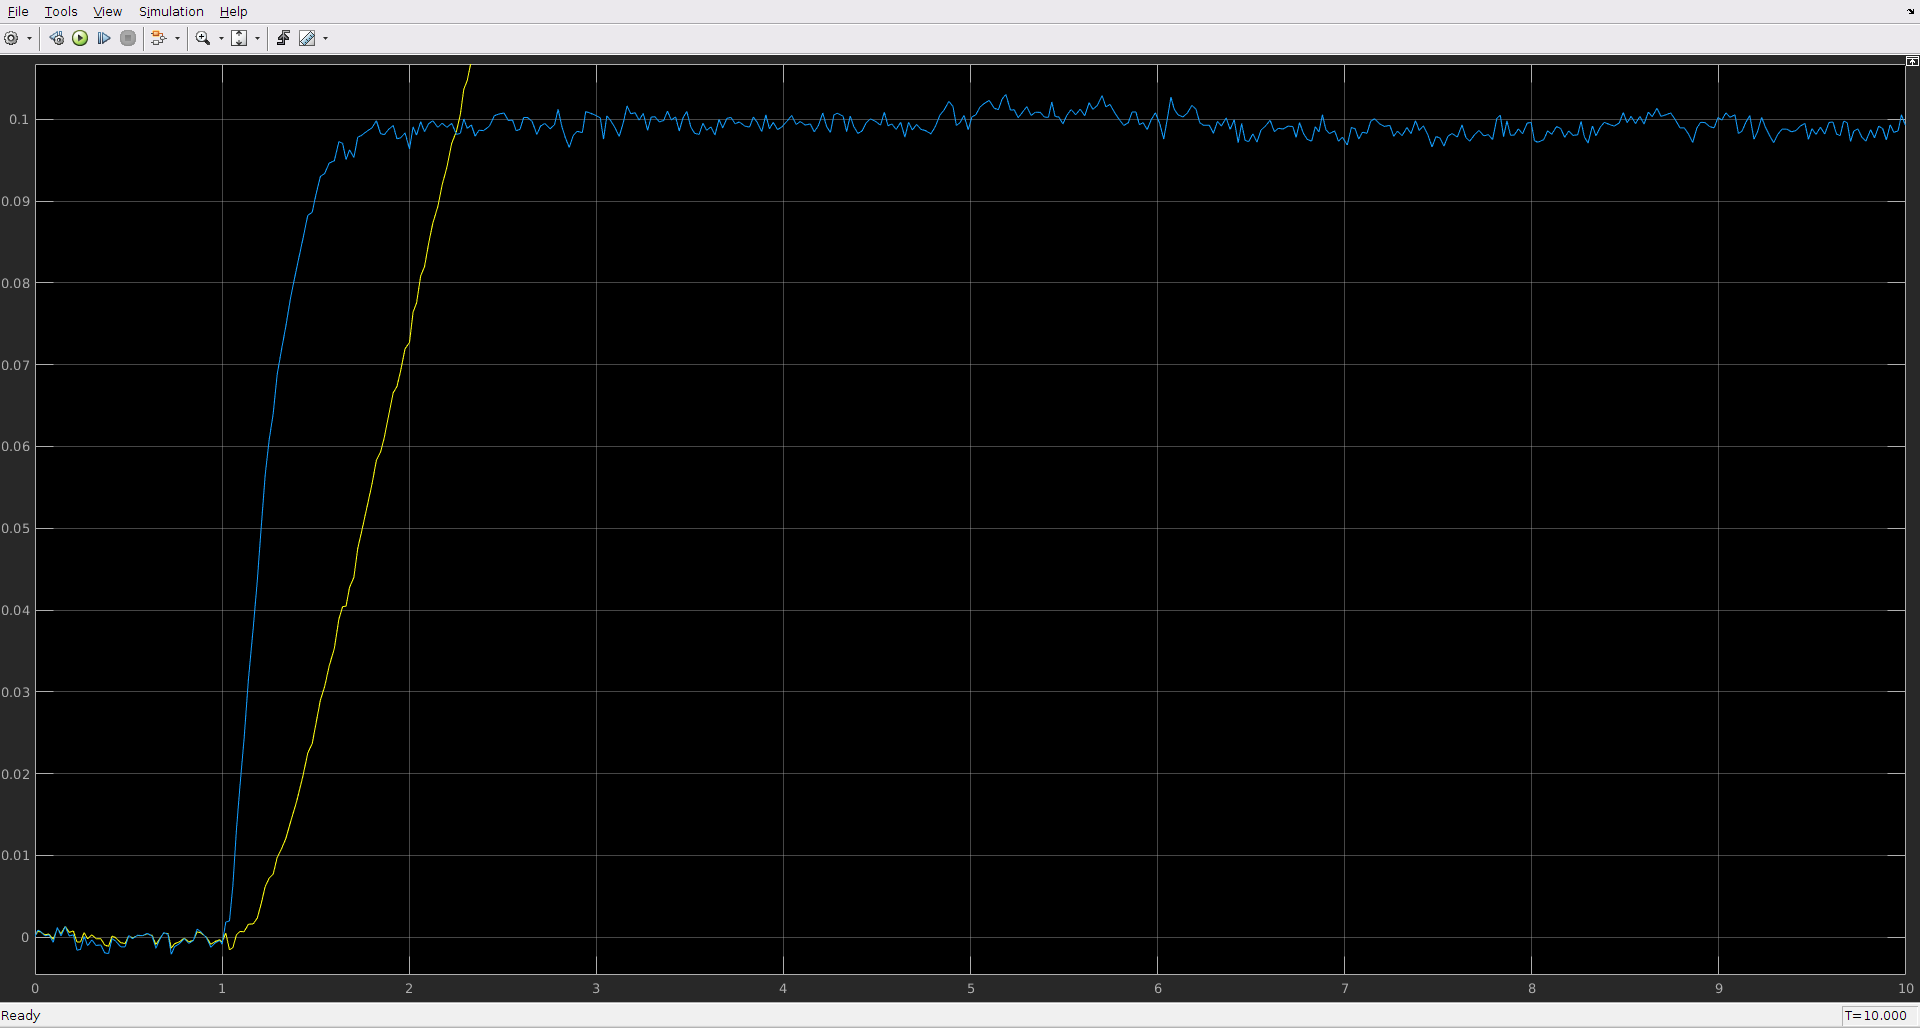
\includegraphics[width=\textwidth]{imglab/lab2sol_identification1.png}
\caption{Typical impulse response for the DCservo model. Omega in blue.}
\label{fig:id1}
\end{figure}

Our model of the DC servo system has an input-speed transfer function
\begin{equation}
	\Omega \left( s \right) = \frac{K_{s}}{\tau s + 1}
\end{equation}
and input-position transfer function
\begin{equation}
	\Theta \left( s \right) = \frac{K_{s}}{s \left( \tau s + 1 \right)}
\end{equation}

 To determine $K_{s}$, we find the steady state value of the step response. By inspection, it seems to be about.1. Noise makes a more precise estimate difficult. We can do some processing to come up with a better estimate. The model created a data structure in the workspace containing the scope data. We can take an a average over the latter part of the data to estimate the steady-state value:
 
\begin{verbatim}
omega = Lab2_Identificationdata.signals(2).values;
avgomega = omega(200:length(omega));
ks = mean(avgomega)
\end{verbatim}

which gives a steady state value of about .0993 in this case. Since our input was a unit step function, our estimate for $K_{s}$ is .0933/1 = .0993. Next, we attempt to estimate $\tau$. First, we find the time at which the response is 63.2\% of its final value, or .0628. We can do this by inspection using the scope's magnification cursor:

\begin{figure}[H]
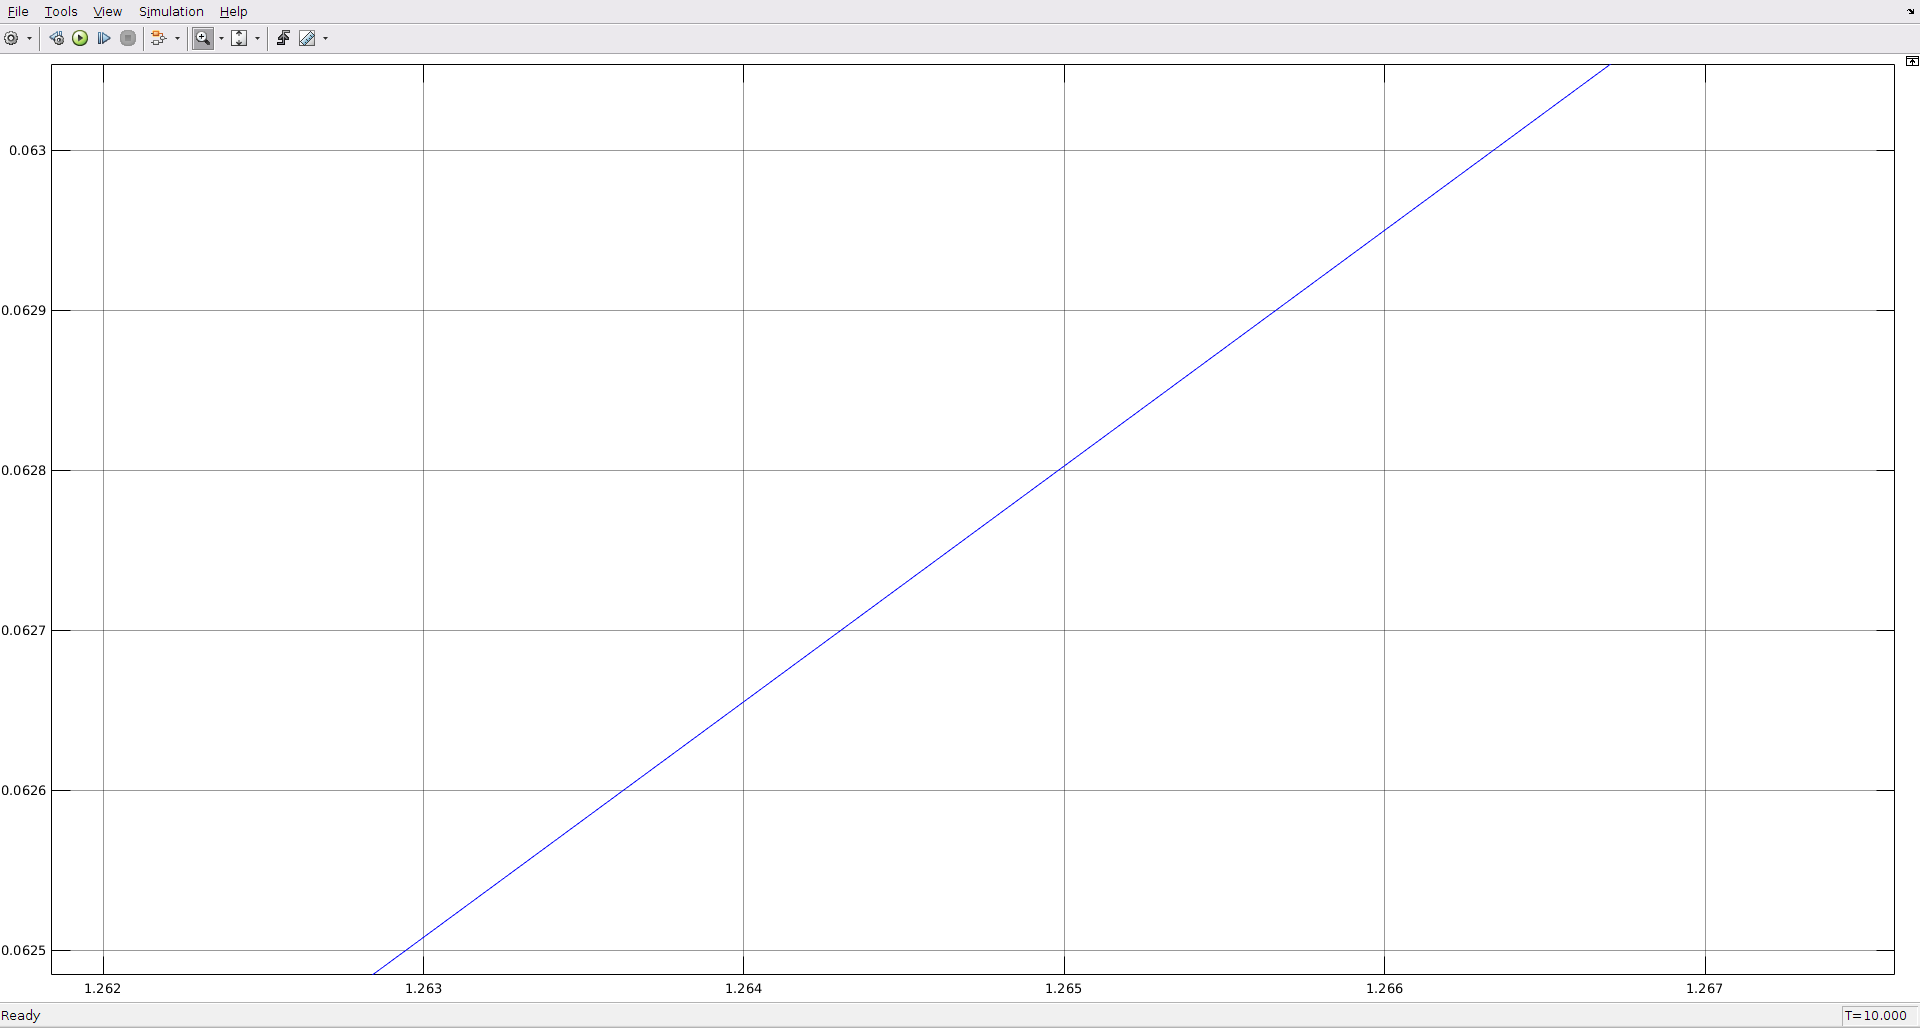
\includegraphics[width=\textwidth]{imglab/lab2sol_identification2white.png}
\caption{Zooming in on the omega trajectory near the point at which it is equal to 63.2\% of the final value. }
\label{fig:id2}
\end{figure}

This time is about 1.265, .265 seconds after the application of the step function. This gives us a value of .265 for $\tau$.

In the Simulink model Lab2\_Comparison, we update the transfer function block according the parameters determined for our model of the DC servo system.

\begin{figure}[H]
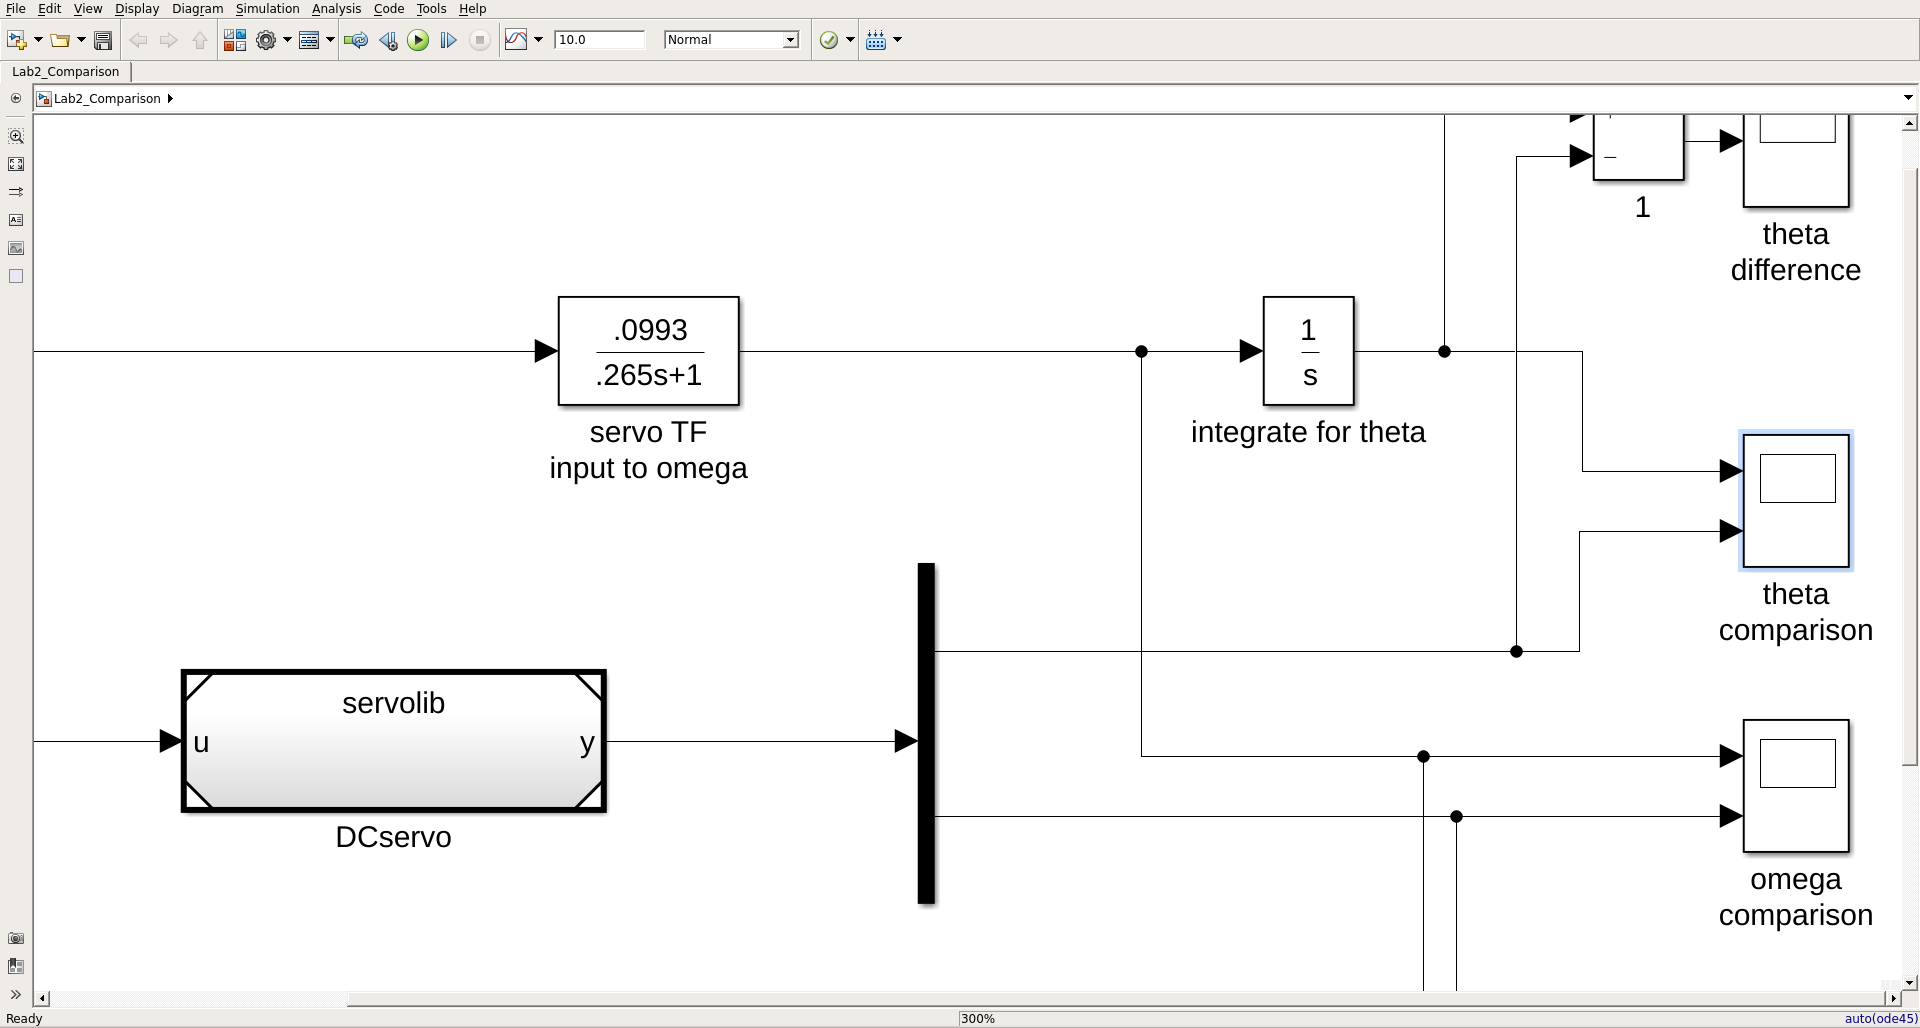
\includegraphics[width=\textwidth]{imglab/lab2sol_comp1.png}
\caption{Lab2\_Comparison.slx with updated model transfer function block. }
\label{fig:comp1}
\end{figure}

We compare the velocity trajectory of our model to that of the DC servo system. 

\begin{figure}[H]
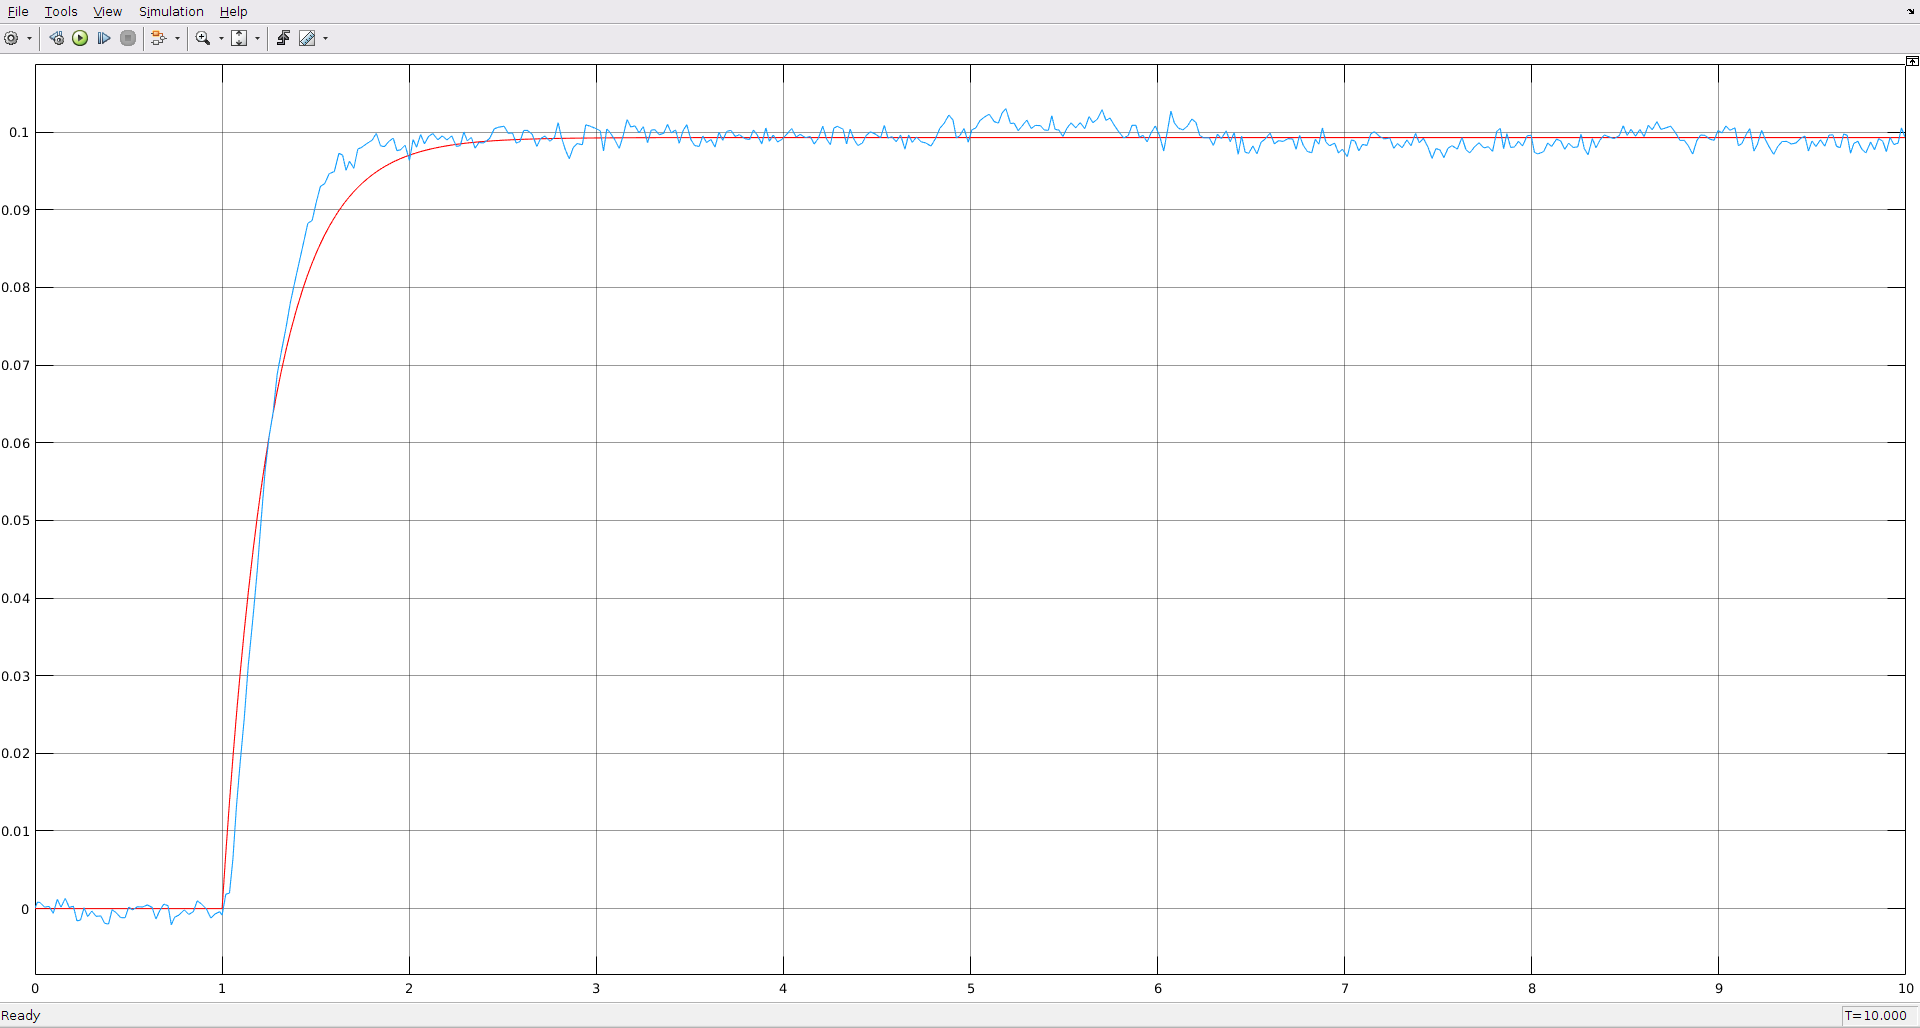
\includegraphics[width=\textwidth]{imglab/lab2sol_comp2.png}
\caption{Omega trajectory comparison. Our model in red and the DC servo system in blue. }
\label{fig:comp2}
\end{figure}

Our model matches the behavior of the system reasonably well, though our model doesn't seem to completely describe the dynamics of the system. Though the curves intersect around one time constant, the model curve is substantially higher before and substantially lower after, until both curves settle at the final value.

\begin{figure}[H]
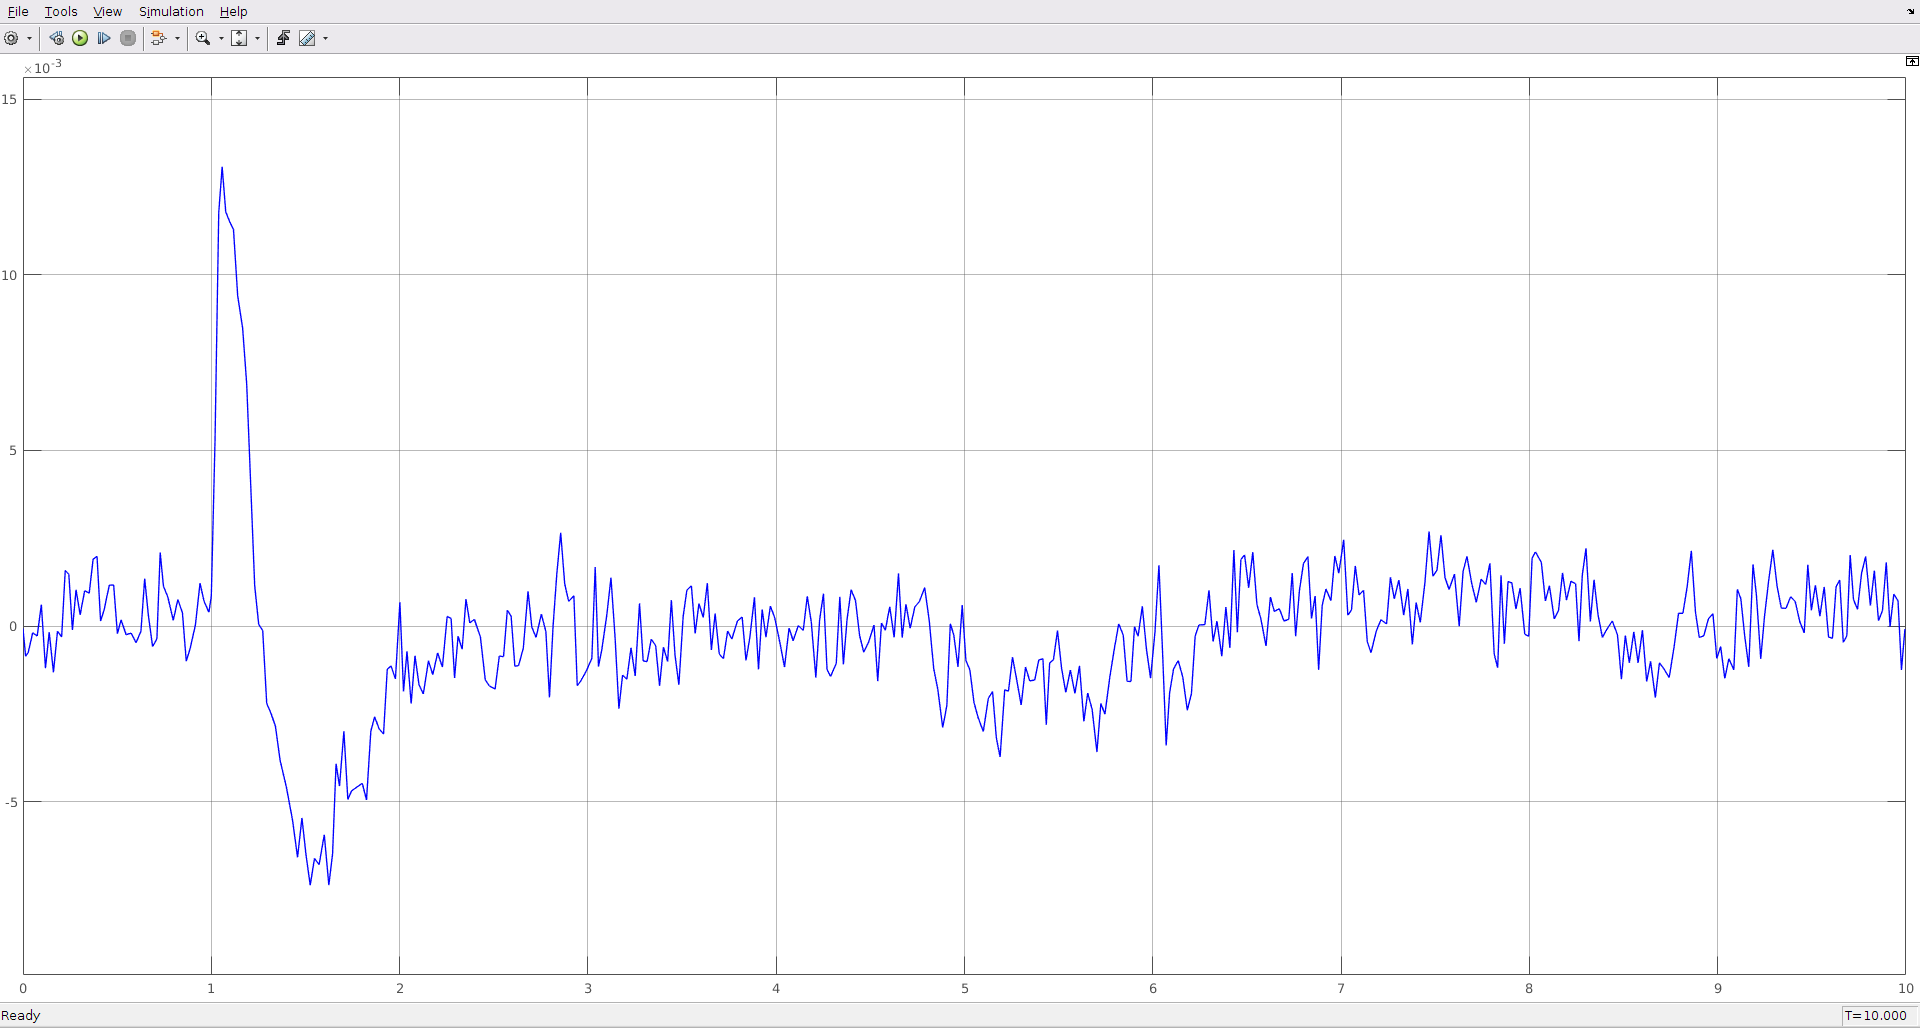
\includegraphics[width=\textwidth]{imglab/lab2sol_mismatch.png}
\caption{The difference in omega trajectories between our model and the system. While not very large, the difference during the rise is greater than can be explained by noise alone. }
\label{fig:comp3}
\end{figure}

It doesn't seem that we can do much better by tweaking parameters, a shorter time constant may reduce error after the curves intersect  at the cost of more error before and vice-versa for a longer time constant. We will stick with the paramter values determined.
\\

\textbf{3.2 Transient Response}

	The model Lab2\_Transient contains 7 DC servo systems each with a different position feedback gain. We run the model, producing a plot with a family of position trajectories:
	
\begin{figure}[H]
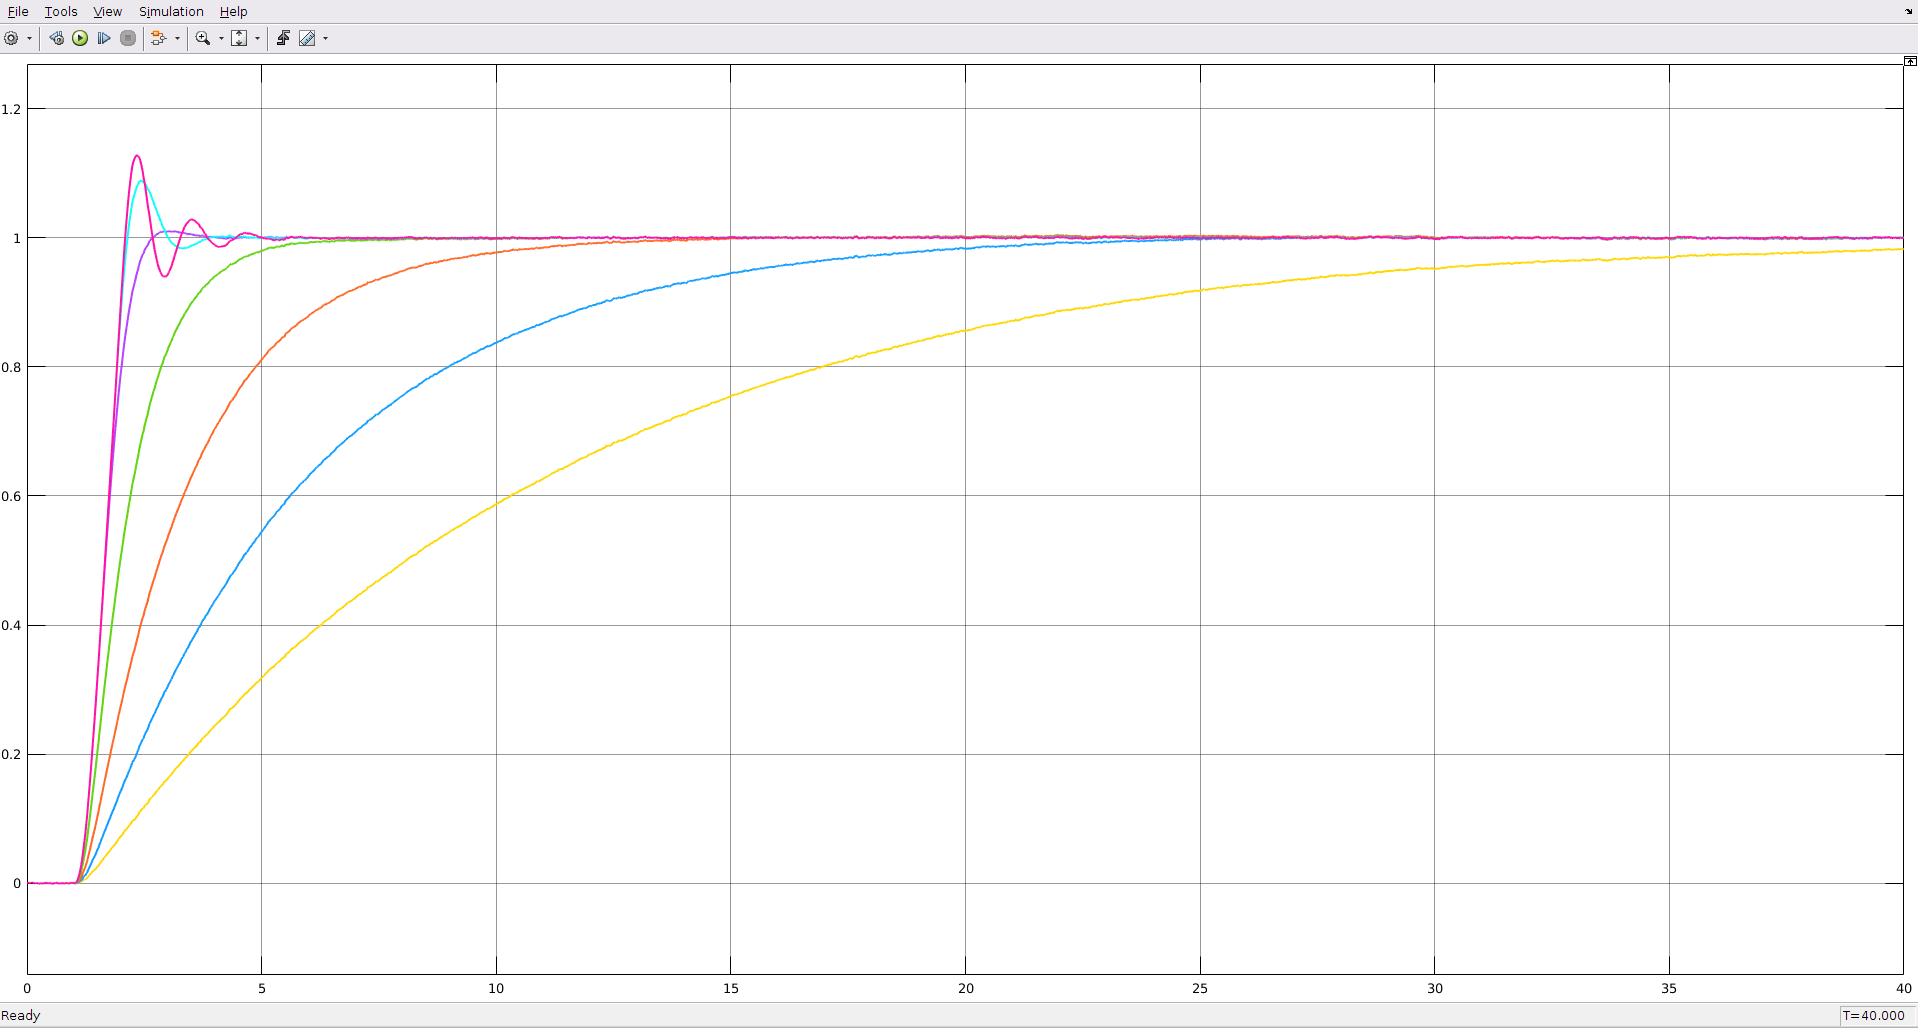
\includegraphics[width=\textwidth]{imglab/lab2sol_transfam.png}
\caption{The family of curves produced from the set of feedback gains (1,2,4,8,16,32,64) with their respective colors yellow, blue, red, green, purple, cyan, and magenta }
\label{fig:transfam}
\end{figure}



\section{Exercises}
\begin{enumerate}

\item From the data of section 3.2, we are able to fill the following table:


\begin{center}
\begin{tabular}{|c|c|c|c|c|c|c|c|}
\hline
Gain & Poles & \%overshoot & $\zeta$ & $\omega_{n}$ & $T_{settling}$ & $T_{peak}$ & $T_{r}$ \\ \hline
1 & -3.67, -.102 & - & 3.08 & .612 & 38.0 & - & 20.9 \\ \hline 
2 & -3.56, -.2103 & - & 2.18 & .866 & 18.2 & - & 10.5 \\ \hline 
4 & -3.32, -.451 & - & 1.55 & 1.22  & 9.3 & - & 4.97 \\ \hline 
8 & -2.64, -1.14 & - & 1.09 & 1.73  & 4.01 & - & 2.17 \\ \hline 
16 & -1.89 $\pm$ 1.56i & 1 & .7706 & 2.45 & 1.50 & 2.03 & 1.68 \\ \hline 
32 & -1.89 $\pm$ 2.90i & 9 & .545 & 3.46 & 2.22 & 1.44 & 1.14 \\ \hline 
64 & -1.89 $\pm$ 4.52i & 13 & .385 & 4.90 & 2.84 & 1.35 & 1.09 \\ \hline 

\end{tabular}
\end{center}

The gain values were read from the Simulink model diagram. The poles were calculated from our model transfer function. For a system with transfer function $\Theta(s)$, the closed loop transfer function with error feedback gain $K_{1}$ is given by:

\begin{equation}
	\frac{K\Theta(s)}{1+K\Theta(s)}
\end{equation}

the following MATLAB script was used to calculate the poles of the closed loop transfer function for each gain.

\begin{verbatim}
	%define constants
	ks = .0993;
	tau = .265;
	K = [1,2,4,8,16,32,64];

	%create transfer function object
	s = tf('s');
	systf = ks/(s*(tau*s + 1));

	%for each gain value
	for i = 1:length(K)
		%find the closed loop transfer function
    	fbsystf = feedback(K(i)*systf,1);
    	display(['poles for ' num2str(K(i)) ' : '])
    	%calculate poles for closed loop system
    	pole(fbsystf)
	end
\end{verbatim}


The percent overshoot was measured by inspection using the scope.

 Our second order transfer function has the form:

\begin{equation}
	G(s) = \frac{\omega_{n}^{2}}{s^{2}+2\zeta\omega_{n}s+\omega_{n}^{2}}
\end{equation}

From $\frac{K\Theta(s)}{1+K\Theta(s)}$ we also have:

\begin{equation}
	G(s) = \frac{\frac{K_{1}K_{s}}{\tau}}{s^{2}+\frac{1}{\tau}s+\frac{K_{1}K_{s}}{\tau}}
\end{equation}


leading to the following formulae for $\zeta$ and $\omega_{n}$:
\begin{equation}
	\omega_{n} = \sqrt{\frac{K_{1}K_{s}}{\tau}}
\end{equation}

\begin{equation}
	\zeta = \frac{1}{2\sqrt{\tau K_{1} K_{s}}}
\end{equation}


$T_{settling}$ is the elapsed time between settling within the 2\% band and the application of the input. $T_{peak}$ is the elapsed time between attainment of the maximum value and application of the input. $T_{peak}$ is only defined for underdamped systems. $T_{r}$ is the rise time, defined for underdamped systems as the elapsed time between first attainment of the target value and the application of the input, and for critically or overdamped systems as $T_{r1}$, the elapsed time between attainment of the 90\% and 10\% values. All of these values were determined by inspection using the scope. 

We also calculated the settling times using the second order model, taking the 2\%s settling time to be about 4 time constants. For an underdamped system the time constant is $\frac{1}{\zeta \omega_{n}}$ and for an overdamped system it is approximately the inverse of the absolute value of the closed loop system's dominant pole.


\item \textbf{(a) Poles plotted in the s-plane for all values of K}

\begin{figure}[H]
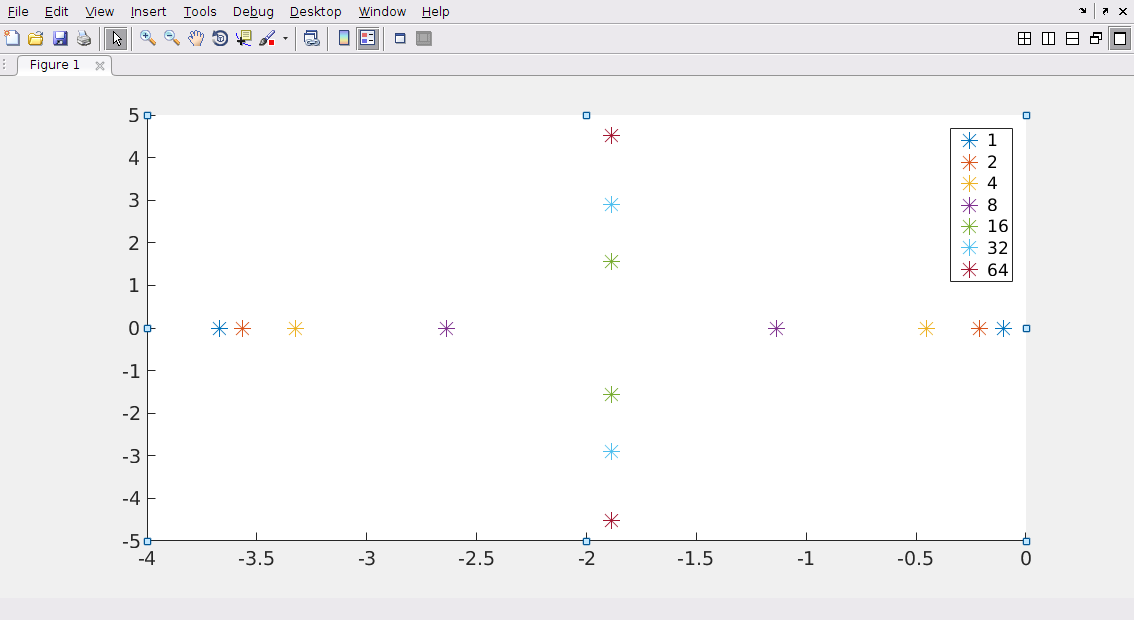
\includegraphics[width=\textwidth]{imglab/lab2sol_ex2a.png}
\caption{Closed-loop poles for all values of K. }
\label{fig:ex2a}
\end{figure}

\textbf{(b) $\zeta$ plotted vs $K_{1}$}
\begin{figure}[H]
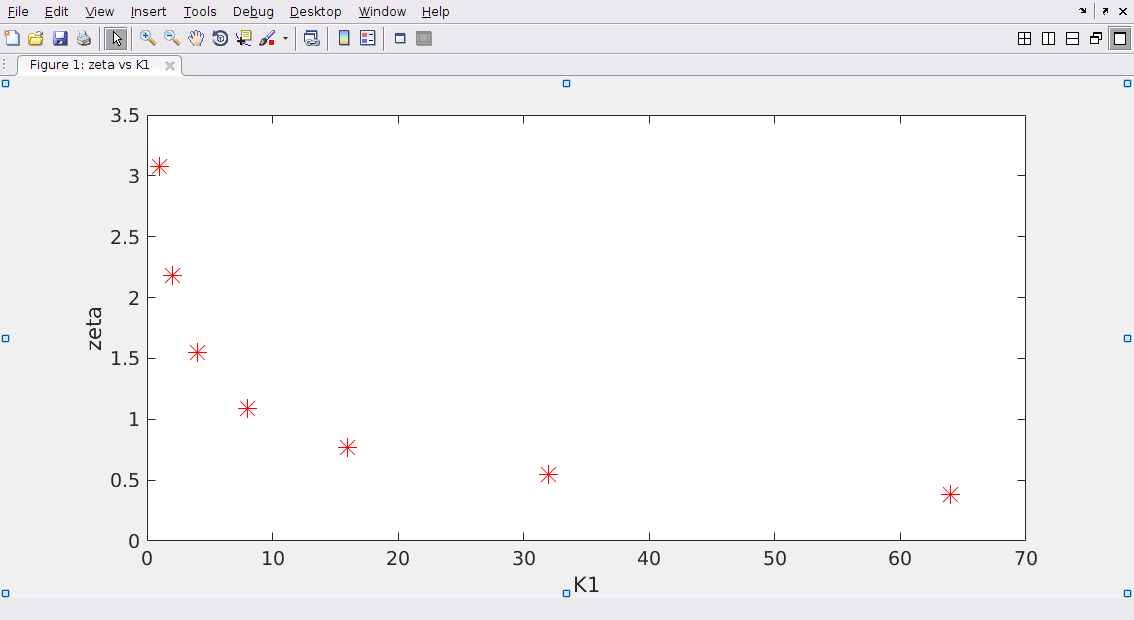
\includegraphics[width=\textwidth]{imglab/lab2sol_zetavsk.png}
\caption{$\zeta$ vs $K_{1}$. }
\label{fig:zetavsk}
\end{figure}

\textbf{(c) \% overshoot plotted vs $\zeta$}
\begin{figure}[H]
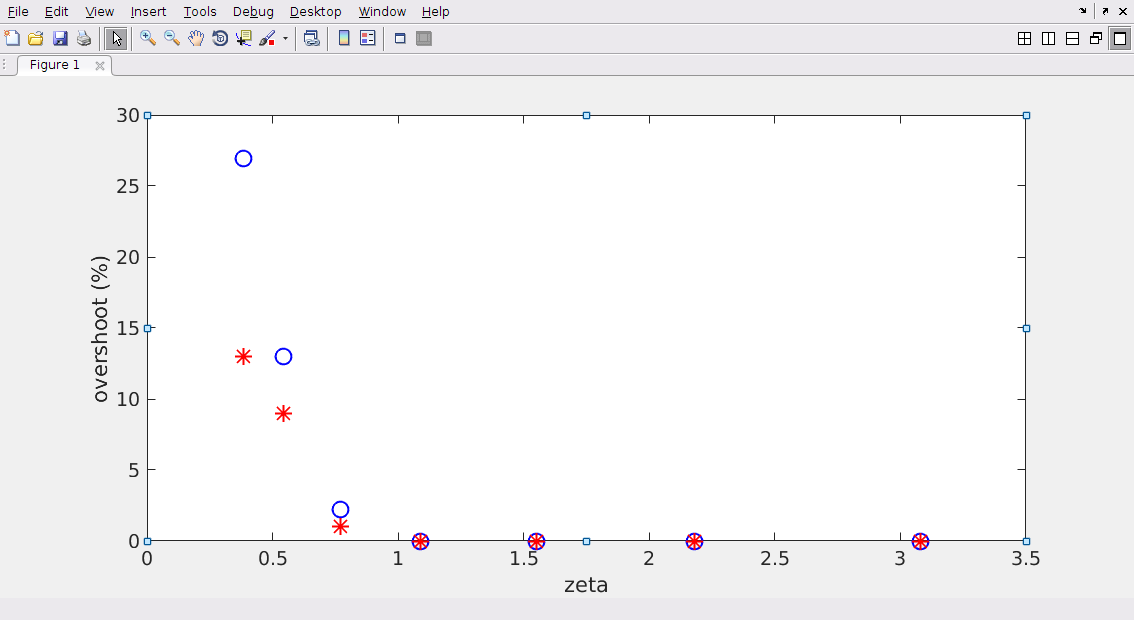
\includegraphics[width=\textwidth]{imglab/lab2sol_osvszeta.png}
\caption{Overshoot vs. $\zeta$. Measured values are red stars, values calculated from model are blue circles. }
\label{fig:osvszeta}
\end{figure}

Measured values are significantly lower than predicted from the second order model. This is due to a saturation block in the model that limits the control effort, modelling the supply voltage of the motor driver. Rise time and peak time are also affected by this factor. This supply voltage will probably be increased in future labs. 

\textbf{(d) settling time vs $\zeta$}
\begin{figure}[H]
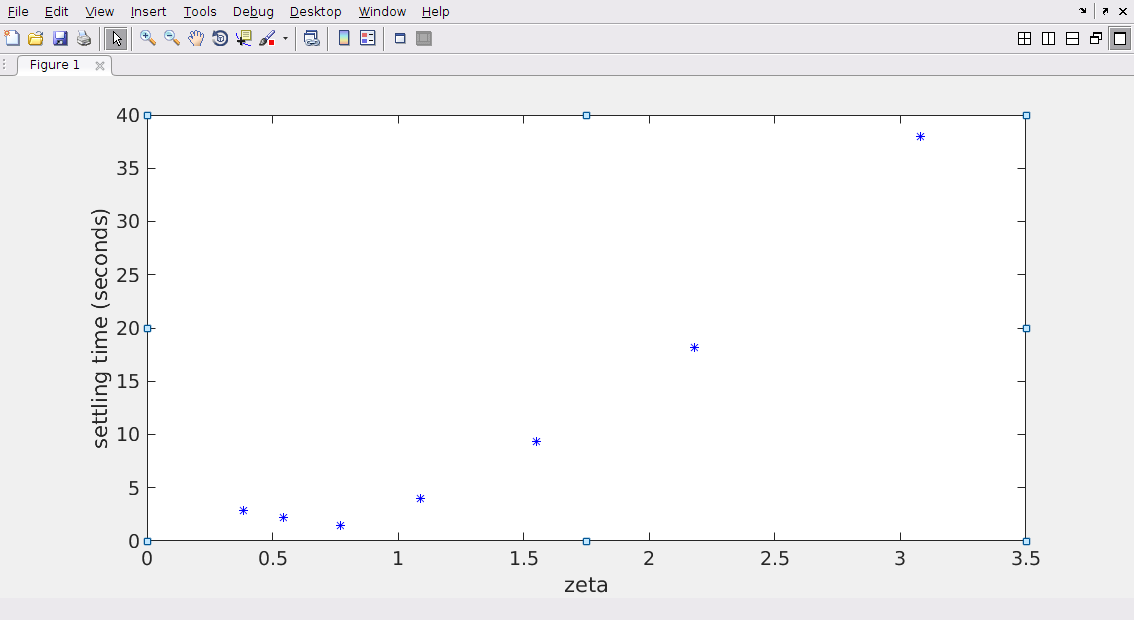
\includegraphics[width=\textwidth]{imglab/lab2sol_stvszeta.png}
\caption{settling time vs. $\zeta$. Measured values are red stars, values calculated from model are blue circles.}
\label{fig:stvszeta}
\end{figure}

\item 

\textbf{(a)} Increasing $K_{1}$ pulls the closed loop poles from their open loop locations on the real axis toward each other. Where they meet, they diverge parallel to the imaginary axis as $K_{1}$ continues to increase.

\textbf{(b)} There is no overshoot until a critical value of $K_{1}$ is reached, at which point the overshoot increases with $K_{1}$.

\textbf{(c)} For an overdamped system, settling time decreases with increasing $K_{1}$. As the gain increases, the system becomes underdamped and the settling time is fixed. 

\end{enumerate}



\end{document}